\qrchapter{https://forgottenpillar.com/rsc/sw-fp-chapter8}{Ukosoaji wa kujenga}

Pointi ya kwanza la \emcap{Kanuni za Msingi} hujibu maswali: Mungu ni nani, ni nini \emcap{Umbile} Wake, na tunaelewaje uwepo Wake?

\others{I. Kwamba kuna \textbf{Mungu mmoja}, \textbf{ \textbf{\underline{huluki}} binafsi wa kiroho}, \textbf{Muumba wa vitu vyote}, mwenye uwezo wote, anayejua yote, na wa milele; Asiye na kikomo katika hekima, utakatifu, haki, wema, ukweli, na rehema; asiyebadilika, na \textbf{kila mahali akiwepo kwa mbinu ya mwakilishi wake, Roho Mtakatifu}. Zab. 139:7.}[FP1889 147.2; 1889][https://egwwritings.org/read?panels=p931.6]

Mungu mmoja, Muumba, anatambulika kama Baba, kwa sababu jambo la pili la \emcap{Kanuni za Msingi} linasema kwamba Yesu Kristo, Mwana wa Baba wa Milele, ndiye pekee ambaye Mungu aliumba vitu vyote\footnote{\href{https://egwwritings.org/?ref=en_FP1889.147.3&para=931.7}{FP1889 147.3; 1889}}. \emcap{Umbile la Mungu} unaonyeshwa katika neno “\textit{huluki binafsi wa kiroho}”. Hivi karibuni tutaona kwamba neno hili linamaanisha kwamba Baba ana mwili wa kimwili, udhihirisho wa kimwili. Kwa hivyo, katika Umbile Lake, Yeye yuko pale tu Anapokaa kimwili. Lakini, Uwepo Wake hauzuiliwi kwa Umbile Lake kwa sababu Yeye \others{yupo kila mahali kupitia mwakilishi wake, Roho Mtakatifu}. Wakati wa historia yetu iliyopita, ufahamu huu na hoja ya \emcap{Umbile la Mungu}, kama inavyoonyeshwa katika nukta ya kwanza ya \emcap{Kanuni za Msingi}, kulipokea ukosoaji wa kujenga; kwa “ukosoaji unaojenga” tunarejelea ukosoaji unaoungwa mkono na Biblia.

Sasa tunakuletea manukuu yafuatayo, ukosoaji fulani wenye kujenga, kutoka kwa ndugu mashuhuri katika shirika la Waadventista Wasabato. Inashangaza, alikuwa amekubali mamlaka ya \emcap{Kanuni za Msingi}, lakini wakati huo huo aliamini mafundisho ya utatu. Tunaona waraka huu kuwa kipengele muhimu sana katika mabadiliko ya imani zetu kutoka kanuni za msingi kuelekea kwa imani ya sasa ya Utatu wa Waadventista Wasabato.

Ndugu huyu mashuhuri alikutanishwa na swali, “\textit{Je, unaamini katika Mungu binafsi, aliye dhahiri?}”:

\others{\textbf{Hakika. Huluki usio na mwisho, na wa kimungu, vilevile wa kibinafsi ni dini muhimu}. Ibada inahitaji Nafsi wa kumpenda, kutii, na kuamini. \textbf{Imani katika Mungu wa kibinafsi ndio msingi wa dini ya Kikristo}. Dhana ya Mungu kama Nishati-Yote, Nguvu isiyo na kikomo, Uwepo unaoenea kote, ni kubwa sana kwa akili ya mwanadamu kushika; lazima kuna kitu \textbf{inayoshikika} zaidi, \textbf{\underline{iliyowekewa vikwazo}} zaidi, ambayo kwayo akili itaegemea katika ibada. \textbf{Ni kwa sababu hii ndiposa Kristo alikuja kwetu kwa mfano wa }\textbf{\underline{Umbile}} \textbf{wa Mungu, Adamu wa pili, ili atuonyeshe kwa maisha yake ya upendo na ya kujitolea tabia na }\textbf{\underline{Umbile la Mungu}}. Tunaweza kumkaribia Mungu kupitia Kristo pekee.}

\othersnogap{‘Ambaye kwa kuwa ni mng'ao wa utukufu wake, na \textbf{chapa halisi ya nafsi yake}, na akivichukua vyote kwa neno la uweza wake, akiisha kufanya utakaso wa dhambi, akaketi chini kwenye mkono wa kuume wa Ukuu huko juu.’}

\othersnogap{‘Ambaye kwa kuwa ni mng'ao wa utukufu wake, na chapa ya asili yake, na kuvitegemeza mambo yote kwa neno la uweza wake.’}

\othersnogap{Mtume asema, ‘Lakini sisi sote, kwa uso usiotiwa utaji, \textbf{tukiurudisha utukufu wa Bwana, kama vile katika kioo}, tunabadilishwa tufanane na mfano uo huo, toka utukufu hata utukufu, kama vile kwa Roho wa Bwana.’ 2 Kor. 3:18. Jinsi sura hii inavyofaa na ya kupendeza!... Kwa hiyo, \textbf{katika kumtazama Kristo} katika miujiza yake, majaribu, mawaidha yake, maisha yake ya kujinyima, ‘kuzunguka-zunguka akitenda mema,’ \textbf{tunaweza kuona Umbile na nguvu za Mungu}. Na kuna tumaini kubwa kiasi kipi kwetu katika ukweli kwamba \textbf{kwa Kristo tunapata sifa ambazo si ngeni na si za kukosa uwiano na za wanadamu}, bali sifa zenye ujamaa moja nasi kiakili na maadili; ili tuweze kuona na kufahamu jambo halisi, badala tu ya ukweli wa kitheolojia au wa kufikirika au wa mfano, katika tamko la mtume, ‘Sasa sisi wana wa Mungu.’ 1 Yohana 3:2.}

\othersnogap{\textbf{Ukweli kwamba Mungu ni mkuu sana hivi kwamba hatuwezi kuwazia waziwazi akilini mwonekano wa }\textbf{\underline{kimwili}}\textbf{ hauhitaji kupunguza katika akili zetu ukweli wa }\textbf{\underline{Umbile Lake}}\textbf{, wala dhana hii haikubaliani na ile ya usemi maalum wa Mungu katika }\textbf{\underline{fomu fulani au mahali fulani}}. \textbf{\underline{Hakika yapo maandiko yanayomtambulisha Mungu katika umbo dhahiri, na mtu anaweza kusema njia ya kuzuiliwa, kama kuketi juu ya kiti cha enzi mbinguni, au kama akikaa katika hekalu la Yerusalemu}}, 1. Wafalme 22:19; Zab. 11:4; Mt. 21:12, 13.}

\othersnogap{Akili ya mwanadamu ina kikomo na haiwezi kutafakari na kuelewa kisicho na kikomo. \textbf{Kwa kawaida tunatamani kuunda kwa uhakika, kwa dhana iliyofafanuliwa waziwazi ya huluki tunayemwabudu}. \textbf{Biblia inapatanisha hitaji hili la mwanadamu na vile vile mahitaji yetu mengine yote ya kiroho, na }\textbf{\underline{katika sura ya arubaini ya Isaya}}\textbf{ nabii anashughulikia swali hili la mwonekano wa kibinafsi ya Mungu kwa namna ya ajabu}. ‘Ee Yerusalemu, uletao habari njema, paza sauti yako kwa nguvu; inueni, msiogope; iambie miji ya Yuda, \textbf{Tazameni, Mungu wenu}! Atalilisha kundi lake kama mchungaji: atawakusanya wana-kondoo mikononi mwake, na kuwachukua kifuani mwake.’}

\othersnogap{‘Ni nani aliyepima maji katika tundu la \textbf{mkono wake}, na kuzipima mbingu kwa morita, na kuyashika mavumbi ya ardhi kwa kipimo, na kuyapima milima ndani ya mizani, na vilima katika mizani? \textbf{Mtamfananisha Mungu na nani basi?} \textbf{Au itakuwa mfano gani mnalinganisha naye?} Je! hamjui? hamjasikia? hamjaambiwa tangu mwanzo? hamjaelewa tangu kuwekwa misingi ya dunia? \textbf{Ni yeye huyo ameketi juu ya duara ya dunia}, na wakaaji wake ni kama panzi; \textbf{hivyo huzitandaza mbingu kama pazia, na kuzitandaza kama hema ya kukaa}: \textbf{\underline{Mtanifananisha na nani basi, au niwe sawa na nani? Asema Mtakatifu}}. Inua macho yako juu, na tazama, ni nani aliyeviumba hivi, yeye aletaye nje jeshi lao kwa hesabu; huwaita wote kwa majina kwa ukuu wa uweza wake, kwa kuwa ana nguvu katika uweza; sivyo mmoja hushindwa. Je, hukujua? hukusikia ya kwamba Mungu wa milele, Bwana, Muumba miisho ya dunia, hazimii wala hachoki? Hakuna kutafuta ufahamu wake. Huwapa nguvu wazimiao na kuwaongeza wasio na uwezo nguvu. Hata vijana watazimia na kuchoka, na vijana wataanguka, lakini wao wamngojeao Bwana watapata nguvu mpya; watapanda juu kwa mbawa kama tai; watapiga mbio, wala hawatachoka; watakwenda kwa miguu, wala hawatazimia.’ Isa. 40:9,11,12,18,21,22,25,26,28-31.}

\othersnogap{\textbf{Hapa kuna maelezo ya ajabu sana ya Mungu. Mkono wake, mkono wake, kifua chake zinatajwa}. Anafafanuliwa kuwa ‘ameketi juu ya duara ya dunia,’ analinganisha mbingu kwa morita, huyashika maji katika tundu la mkono wake; \textbf{\underline{hivyo hakuwezi kuwa na swali kwamba Mungu ni huluki dhahiri, halisi na wa kibinafsi}}. \textbf{Kanuni ya kufikirika tu, sheria, nguvu hawezi kuwa na viganja au mkono. \underline{Mungu ni Nafsi}, ingawa ni mkuu sana kwetu sisi kuelewa, kama Ayubu anasema}, ‘Mungu ni mkuu na sisi hatumjui.’ Ayubu 36:26...}

\othersnogap{\textbf{\underline{Huluki huyu mkubwa} Anawakilishwa kama ameketi kwenye duara la dunia}. Mzunguko wa dunia ina kipenyo cha takriban maili milioni mia mbili. \textbf{Huluki mkubwa sana hadi kuchukua kiti cha namna hiyo ni \underline{zaidi ya ufahamu wetu kuhusu umbo lake}}. \textbf{Nabii anatambua hili, na hivyo \underline{kugeuza mawazo yetu mbali na uvumi kuhusu ukubwa na umbo kamili wa Mungu} kwa kutuonyesha upuuzi wa kujaribu kufanyiza hata picha akilini, \underline{akionyesha kwamba jambo hilo ni sawa kabisa na ibada ya sanamu}. Tazama mistari 18-21}. Kisha anatuonyesha mahali pa kupata wazo la kweli la Mungu, akituelekeza kwenye mambo ambayo ameifanya: ‘Inueni macho yenu juu, mwone ni nani aliyeviumba hivi. Hili pia lilikuwa wazo la Paulo: ‘Kwa maana vitu vyake visivyoonekana tangu kuumbwa ulimwengu vinaonekana waziwazi, ikifahamika kwa vitu vilivyofanyika, \textbf{yaani, uweza wake wa milele na \underline{Uungu}}; ili wasiwe na udhuru.’ Rum. 1:20.}

\othersnogap{\textbf{\underline{Majadiliano yanayohusu umbo la Mungu hayana faida kabisa}, na hutumikia tu kudhalilisha dhana zetu za yeye aliye juu ya vitu vyote}, \textbf{na hivyo haipaswi kulinganishwa kwa umbo au ukubwa au utukufu au ukuu pamoja na kitu chochote ambacho mwanadamu amewahi kukiona au ambacho kicho katika uwezo wake kuuvutia taswira}. Katika uwepo wa maswali kama haya, lazima tu tukiri upumbavu wetu na kutoweza, na tuinamishe vichwa vyetu kwa kicho na heshima \textbf{mbele ya uwepo wa Nafsi, Huluki wenye Akili} uwepo wake ambao kwayo maumbile yote ina ushuhuda wa uhakika na chanya, \textbf{lakini ambaye ni mbali zaidi ya uwezo wa ufahamu wetu \underline{kama vile mipaka ya nafasi na wakati}}.}

Kama ilivyotajwa hapo awali, ndugu huyu anakubali \emcap{Kanuni za Msingi}, lakini analiamini Utatu. Huu hapa ni muhtasari mfupi wa ukosoaji Wake wenye kujenga kuhusu \emcap{ubinafsi wa Mungu}: Mungu ni huluki dhahiri, halisi, binafsi, mwenye umbo—\others{\textbf{Hakika, kuna maandiko ambayo yanamwasilisha Mungu katika \underline{hali hii ya umbo dhahiri}, na mtu anaweza kusema njia ya \underline{kuzuiliwa}, kama ameketi juu ya kiti cha enzi mbinguni}}. Anatetea hili kwa sababu anaamini ni muhimu kwetu, wanadamu wenye ukomo, kuwa na shabaha ya hakika ya kuabudiwa. Lakini anapanua wazo la Mungu “aliyezuiliwa” kwa ushuhuda kutoka kwa Isaya sura ya 40, ambayo inathibitisha kwamba Mungu yuko\others{\textbf{\underline{zaidi ya ufahamu wetu kuhusu umbo lake}}}. Aina yoyote ya dhana ya Mungu kuwa, kwa namna yoyote ile, ni sawa na ibada ya sanamu. \others{\textbf{\underline{Majadiliano yanayohusu umbo la Mungu hayana faida kabisa}}}. Jambo la kweli la ubinafsi wa Mungu asiye na kikomo ni zaidi ya ufahamu wetu. Ubinafsi wa kweli wa Mungu ni zaidi ya fumbo kwa akili zetu zenye kikomo. Hii ni kwa sababu Mungu yuko\others{\textbf{mbali zaidi ya uwezo wa ufahamu wetu \underline{kama vile mipaka ya nafasi na wakati}}}. Kwa ndugu huyu, kuelewa ubinafsi wa Mungu kama Huluki hususa ni kwa njia moja kweli, lakini kwa njia nyingine ni uwongo. Ni kweli kwamba Mungu alijidhihirisha katika \others{\textbf{\underline{fomu au mahali maalum}}}, kwa sababu \others{lazima kuwe na kitu \textbf{kinachoonekana} zaidi, \textbf{\underline{kilichozuiliwa}} zaidi, ambacho kinaweza tegemeza akili katika ibada}. Ufahamu nyepesi wa Mungu kama huluki dhahiri na wa kushikika ni kizuizi kwa Mungu. Muhtasari wa ukosoaji wake ni kwamba tunapaswa kuunda dhana zetu za Mungu nje ya \others{\textbf{mipaka ya nafasi na wakati}}.

Tafadhali, chunguza kwa unyoofu sababu za imani ya ndugu huyu. Mwongozo wa fikira zake ni muhimu kuuelewa kwa sababu ulichukua jukumu muhimu katika Historia ya Waadventista Wasabato, kama hatua ya ujasiri mbali na \emcap{Kanuni za Msingi}. Hoja hizi sio ndogo; unao ushawishi sana na tunakuhimiza utafakari. Labda wewe unaweza kukubaliana nao, lakini tafadhali turuhusu kufichua udanganyifu. Nukuu hizi ni kutoka kwa kitabu cha Dk. Kellogg “The Living Temple”\footnote{\href{https://archive.org/details/J.H.Kellogg.TheLivingTemple1903}{Dr. J. H. Kellogg, The Living Temple, p.29-33.}}. Kutoka kwa sehemu yenye kichwa “Huluki Binafsi Aliye na Ujuzi Bila Kikomo”, ukurasa wa 29 hadi 33, vifungu vinaeleza msimamo wa Kellogg kuhusu \emcap{ubinafsi wa Mungu}, ambalo lilikuwa tatizo kuu la kitabu chake.

Hicho ambacho umesoma hivi punde ndicho hasa Dada White alirejelea aliposema: \egwinline{Ninao mambo machache ya kusema kwa walimu wetu \textbf{yakirejelea kitabu kipya The Living Temple}. \textbf{Kuwa mwangalifu jinsi unavyotegemeza hisia za kitabu hiki \underline{kuhusu ubinafsi wa Mungu}}. Bwana anavyowasilisha mambo kwangu, \textbf{hisia hizi hazikubaliki na Mungu}. \textbf{Ni mtego ambao adui ameutayarisha kwa siku hizi za mwisho}...}[Lt211-1903.1; 1903][https://egwwritings.org/read?panels=p9598.8]

Katika pambano la sasa la Waadventista Wasabato juu ya fundisho la Utatu, kibinafsi tumekuwa tukijaribu kuhamisha utata kutoka kwa fundisho la Utatu hadi \emcap{ubinafsi wa Mungu}. Tumewasilisha msimamo wa hoja ya kwanza ya \emcap{Kanuni za Msingi} na tumekumbana na mabishano ambayo yanaingiliana sana na maoni ya Dk. Kellogg juu ya \emcap{ubinafsi wa Mungu}, yanayotetewa katika “The Living Temple”. Tumeona hili mara kwa mara. Wakati umakini unatolewa kutoka kwa suala la Utatu hadi \emcap{ubinafsi wa Mungu}, maoni ya Kellogg kuhusu \emcap{ubinafsi wa Mungu} mara kwa mara hutoka midomoni mwa watetezi wa Utatu. Ubora au hali ya Mungu kuwa Nafsi ni fumbo katika fundisho la Utatu, na mara nyingi maoni ya Kellogg juu ya \emcap{ubinafsi wa Mungu} inapatana na ufahamu wa Utatu wa nafsi ya Mungu.

\begin{figure}[hp]
    \centering
    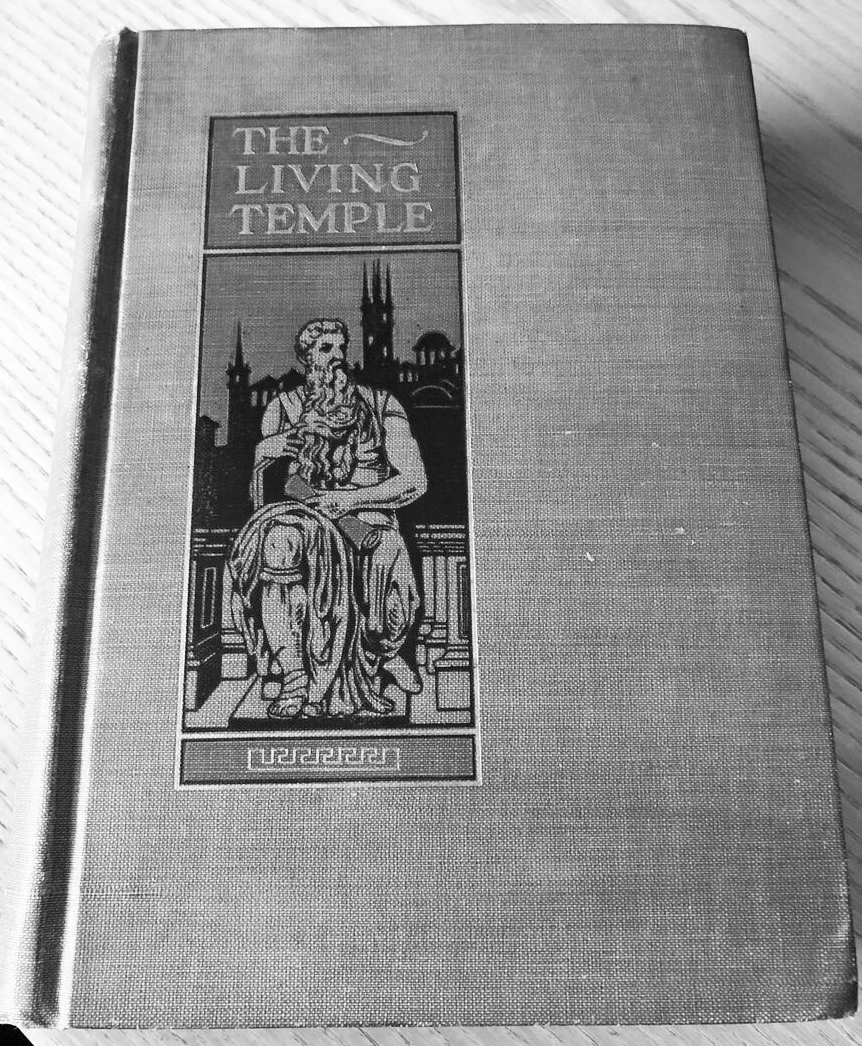
\includegraphics[width=1\linewidth]{images/TLT.jpg}
    \caption*{The Living Temple na Dk. J. H. Kellogg, 1903}
    \label{fig:tlt}
\end{figure}

Baadhi ya watu wanaona ufahamu wa Dk. Kellogg kuhusu Umbile la Mungu unahusiana na uelewa wao, lakini wanashawishika kufikiri kwamba kuna mambo mengine ya kukemewa zaidi katika Hekalu Hai. Ushahidi ufuatao unaonyesha kinyume kabisa. Kuna barua kutoka Dk. Kellogg kwa William C. White, ambapo Dk. Kellogg anapendekeza \others{kukatwa kwa kurasa chache} kutoka kwa nakala elfu tatu za Hekalu Hai—kurasa zile hasa zenye \others{ mambo yenye kuchukiza yanatokea, kama vile maelezo juu ya Isaya 40} na maoni kuhusu \emcap{Umbile la Mungu} (kurasa ambazo tumesoma).

\others{Sanitarium inazo, napata, \textbf{vitabu elfu mbili au elfu tatu ambavyo viliuzwa}, lakini ambavyo vimeregeshwa tangu kitabu kilipokaripiwa. Swali limeulizwa, je! Nini kitafanywa na hivi? \textbf{Wazo limenijia kwamba labda vinaweza kuokolewa \underline{kwa kukata kurasa chache} ambazo \underline{hasa mambo yenye kuchukiza yanatokea}, kama vile \underline{maoni juu ya Isaya 40}, ambayo nilikopa kutoka kwa A.T. Jones, na ukurasa ambao kichwa kisichokusudiwa kinaonekana, ‘\underline{Umbile la Mungu},’ na kupeana kurasa zinazojumuisha taarifa iliyo wazi ya maoni ya Biblia juu ya Mungu kama Nafsi inayotolewa katika Nakala ya Mzee Haskell katika ‘Review’ wiki chache zilizopita}. Vitabu hivi vitauzwa kwa wazee wagonjwa wanaohitaji sana kitabu cha zawadi za Krismasi…}[Letter from Dr. J.H. Kellogg to W.C.White; December 6, 1903, Chicago][https://174625.selcdn.ru/ellenwhite/EWhite/17226/17226.pdf]

Je, ni suala gani la kweli kuhusu hoja zilizowasilishwa katika Hekalu Hai? Tutajifunza suala hilo hadi kwenye mizizi yake; kijuujuu, tunaona wazi kuwa suala ni kuvuka msingi wa imani yetu—\emcap{Kanuni za Kimsingi}—kuhusu \emcap{Umbile la Mungu} na mahali uwepo wake upo.

\egw{\textbf{Nimeagizwa na mjumbe wa mbinguni} kwamba \textbf{baadhi ya hoja} katika kitabu, ‘Hekalu Hai’, hazina msimamo wa kweli na kwamba \textbf{mawazo haya yangepotosha} akili za wale ambao hawajaimarishwa kikamilifu kuhusu \textbf{kanuni za msingi} za ukweli wa sasa. \textbf{Inatanguliza yale ambayo si kitu ila dhana tu} kuhusiana na \textbf{Umbile la Mungu na uwepo wake ulipo}.}[SpTB02 51.3; 1904][https://egwwritings.org/read?panels=p417.262]

Dk. Kellogg alianzisha wazo \egwinline{ambalo si lolote bali ni uvumi kuhusu Umbile la Mungu}, ambayo kwayo alivuka na kutoka kwenye msingi wa imani yetu—\emcap{Kanuni za Kimsingi}. Tofauti kati ya mafundisho ya Dk. Kellogg na \emcap{Kanuni za Kimsingi} iko katika kauli ya kwanza ya kanuni ambapo tunafundishwa kwamba\others{Kwamba kuna \textbf{Mungu mmoja}, \textbf{huluki binafsi wa kiroho}, \textbf{muumba wa vitu vyote}, ... na \textbf{kila mahali akiwepo kwa mwakilishi wake, Roho Mtakatifu}. Zab. 139:7.}

Dada White alituonya moja kwa moja kuhusu maoni yaliyoonyeshwa katika Hekalu Hai kuhusu \emcap{Umbile la Mungu}. Hazipatani na hoja ya kwanza ya \emcap{Kanuni za Kimsingi}, ambayo yalikuwa sehemu ya msingi wa imani yetu.

\egw{\textbf{Nimelazimika kuandika mengi kuhusu mafundisho ya ajabu na nadharia zinazoonyeshwa katika Hekalu Hai. \underline{Ikiwa nadharia hizi zingekubaliwa na watu wetu, nguzo imara za imani yetu na kweli ambazo zimetuwafanya Waadventista Wasabato jinsi walivyo zingefagiliwa mbali}. Nimelazimika kuonyesha uwongo wa mafundisho haya, nikiyawasilisha \underline{kama aina za uzushi wa siku za mwisho}. Tunaambiwa kwa Neno la Mungu kwamba mafundisho kama hayo \underline{yataletwa miongoni mwetu hasa kwa wakati huu}.}}[Lt250-1903.2; 1903][https://egwwritings.org/read?panels=p9337.8]

Leo tunashuhudia kukubalika kwa nadharia za Kellogg kuhusu \emcap{Umbile la Mungu}. Ukweli kwamba hatua ya kwanza ya \emcap{Kanuni za Kimsingi} haipo tena katika imani yetu inathibitisha kwamba nadharia za Kellogg kuhusu \emcap{Umbile la Mungu} zimekuwa na ushawishi katika kutengeneza imani zetu.

\egw{Mmoja na mwingine wanakuja kwangu, wakiniuliza \textbf{nieleze nafasi zilizochukuliwa katika “Hekalu Hai.”} Ninajibu, “Hazielezeki.” \textbf{Maoni yanayotolewa hayatoi ukweli kuhusu maarifa ya Mungu.} \textbf{Katika kitabu chote kuna vifungu vya maandiko}. \textbf{Maandiko haya yanaletwa kwa njia ambayo \underline{kosa linafanywa lionekane kuwa kweli}}. \textbf{Nadharia potofu zinawasilishwa kwa njia ya kupendeza sana hivi kwamba isipokuwa uangalifu unachukuliwa, wengi watapotoshwa}.}[SpTB02 52.1; 1904][https://egwwritings.org/read?panels=p417.265]

Kosa linafanywa lionekane kuwa kweli, na wengi wamepotoshwa.

Inafaa kusisitiza, kwa msomaji fulani asiyemakinika, kwamba suala halisi la Dk. Kellogg, na kitabu chake “\textit{Living Temple}”, si Utatu bali ni hatua ndogo aliyoichukua kutoka kwenye \emcap{Kanuni za Msingi}. Ili kuelewa suala halisi la kitabu chake, itakuwa ni makosa kuzingatia hisia zake zinazopishana na fundisho la Utatu. Badala yake, tunapaswa kuzingatia jambo hilo likijumuisha hatua hii ndogo aliyoichukua; na hii ni pamoja na kuwa na uelewa wa kina wa \emcap{kanuni za msingi} kama vile waanzilishi wetu walivyokuwa nao. Nani bora kuuliza isipokuwa Waadventista waanzilishi wenyewe?

% Constructive Criticism

\begin{titledpoem}
    
    \stanza{
        A personal God in heaven sits enthroned, \\
        This truth in our Principles firmly zoned. \\
        Present everywhere by Spirit's might, \\
        This foundation stood as our guiding light.
    }

    \stanza{
        Then came words that seemed so wise and deep, \\
        A subtle shift that made the faithful weep. \\
        "God's form beyond all human thought," they claimed, \\
        A mystery too vast to be contained or named.
    }

    \stanza{
        "Discussions of God's form," the Temple said, \\
        "Are futile paths where idols lie ahead." \\
        Yet this philosophy so smoothly spun, \\
        Was the very snare by which souls were won.
    }

    \stanza{
        The error dressed as truth appeared so fair, \\
        As scripture twisted in a clever snare. \\
        One small step from the Principles we held, \\
        One giant leap by which our faith was felled.
    }

    \stanza{
        Beware the mind that thinks itself too wise, \\
        To see deception veiled in truth's disguise. \\
        God is personal, definite, and real, \\
        This is the truth the Temple would conceal. 
    }
\end{titledpoem}
